% Options for packages loaded elsewhere
\PassOptionsToPackage{unicode}{hyperref}
\PassOptionsToPackage{hyphens}{url}
%
\documentclass[
]{article}
\usepackage{amsmath,amssymb}
\usepackage{iftex}
\ifPDFTeX
  \usepackage[T1]{fontenc}
  \usepackage[utf8]{inputenc}
  \usepackage{textcomp} % provide euro and other symbols
\else % if luatex or xetex
  \usepackage{unicode-math} % this also loads fontspec
  \defaultfontfeatures{Scale=MatchLowercase}
  \defaultfontfeatures[\rmfamily]{Ligatures=TeX,Scale=1}
\fi
\usepackage{lmodern}
\ifPDFTeX\else
  % xetex/luatex font selection
\fi
% Use upquote if available, for straight quotes in verbatim environments
\IfFileExists{upquote.sty}{\usepackage{upquote}}{}
\IfFileExists{microtype.sty}{% use microtype if available
  \usepackage[]{microtype}
  \UseMicrotypeSet[protrusion]{basicmath} % disable protrusion for tt fonts
}{}
\makeatletter
\@ifundefined{KOMAClassName}{% if non-KOMA class
  \IfFileExists{parskip.sty}{%
    \usepackage{parskip}
  }{% else
    \setlength{\parindent}{0pt}
    \setlength{\parskip}{6pt plus 2pt minus 1pt}}
}{% if KOMA class
  \KOMAoptions{parskip=half}}
\makeatother
\usepackage{xcolor}
\usepackage[margin=1in]{geometry}
\usepackage{graphicx}
\makeatletter
\def\maxwidth{\ifdim\Gin@nat@width>\linewidth\linewidth\else\Gin@nat@width\fi}
\def\maxheight{\ifdim\Gin@nat@height>\textheight\textheight\else\Gin@nat@height\fi}
\makeatother
% Scale images if necessary, so that they will not overflow the page
% margins by default, and it is still possible to overwrite the defaults
% using explicit options in \includegraphics[width, height, ...]{}
\setkeys{Gin}{width=\maxwidth,height=\maxheight,keepaspectratio}
% Set default figure placement to htbp
\makeatletter
\def\fps@figure{htbp}
\makeatother
\setlength{\emergencystretch}{3em} % prevent overfull lines
\providecommand{\tightlist}{%
  \setlength{\itemsep}{0pt}\setlength{\parskip}{0pt}}
\setcounter{secnumdepth}{-\maxdimen} % remove section numbering
\ifLuaTeX
  \usepackage{selnolig}  % disable illegal ligatures
\fi
\IfFileExists{bookmark.sty}{\usepackage{bookmark}}{\usepackage{hyperref}}
\IfFileExists{xurl.sty}{\usepackage{xurl}}{} % add URL line breaks if available
\urlstyle{same}
\hypersetup{
  pdftitle={Summary},
  pdfauthor={JM and HN},
  hidelinks,
  pdfcreator={LaTeX via pandoc}}

\title{Summary}
\author{JM and HN}
\date{2023-08-11}

\begin{document}
\maketitle

\hypertarget{what-we-have-done-so-far}{%
\section{What we have done so far:}\label{what-we-have-done-so-far}}

\hypertarget{fragmented-theoretical-background}{%
\subsection{Fragmented theoretical
background:}\label{fragmented-theoretical-background}}

\hypertarget{topic-one-discussed-in-this-summary}{%
\subparagraph{Topic one (discussed in this
summary):}\label{topic-one-discussed-in-this-summary}}

When assessing decision algorithms one must consider whether making a
decision at all is advisable. For instance, in scenarios where the
consequences of incorrect decisions are substantial, it might be more
prudent not to make a decision or categorize cases with missing
information regarding critical predictors.

Measuring the effectiveness of potential decision rules is achieved most
effectively by calculating expected costs.

To explore situations where not making a decision may be preferable to
deciding under uncertainty, we conducted a comparative analysis of
FFTrees' performance under four conditions: handling complete
information, handling incomplete information with the FFTrees package,
and utilizing two strategies of not-deciding in analogous scenarios.

\hypertarget{topic-two-will-hopefully-be-investigated-in-the-future}{%
\subparagraph{Topic two (Will hopefully be investigated in the
future):}\label{topic-two-will-hopefully-be-investigated-in-the-future}}

Comparisons between fast and frugal heuristics and other decision
algorithms have demonstrated that in uncertain environments, the former
often yield predictions as accurate as those from less frugal algorithms
(Phillips et al., 2017).

We hypothesize that the frugal nature of FFTrees confers a comparative
advantage in handling incomplete data sets, making it robust in dealing
with real-world uncertainties (Gigerenzer \& Gaissmaier, 2011). This is
particularly relevant given the persistent presence of uncertainty in
everyday life.

In future research, we aim to delve deeper into how various algorithms
handle similar amounts of missing data and determine which algorithm
demonstrates the highest level of robustness in such circumstances.

\hypertarget{tools}{%
\subsection{Tools:}\label{tools}}

Aside from using the R package ``FFTrees'', the functions
``replace\_values'', ``loop\_NA'', ``loop\_pc'' and ``loop\_datasets''
were developed in order to randomly add defined percentages of NAs to
specific variables of multiple data sets. Also, then the best FFTree of
the original data set is applied to several randomly developed ``NA-data
sets'' and it is tested how well the criterion is predicted on average
with a given percentage of NAs.

\hypertarget{method}{%
\subsection{Method:}\label{method}}

Regarding topic one, we computed the performance of FFTrees algorithms
across multiple data sets, utilizing the original best tree for all
subsequent investigations.

We then investigated the performance of a ``one\_IDK'' option, that
would classify all cases as ``I don't know'' that had missings in all
nodes of the ``best tree''. (Calculation to determine the number of
``IDK'' cases: percentage \textless- pc of NAs\^{}nodes)

We further had a look on the performance of the ``all\_IDK'' option
which would decide ``I don't know'' for a case as soon as there was a
missing value in any of the variables used at the nodes. (Calculation to
determine the number of ``IDK'' cases: percentage \textless- pc + (1 -
pc) * pc + (1 - pc) * (1 - pc) * pc)

Lastly, we assessed the performance of our conventional approach to
managing missing data within the FFTree algorithm.

All performances were compared for their costs: Costs of a right
decision were held constant with -1. Costs of an ``IDK'' were held
constant with 0 and costs of a wrong decision were the x-variable that
was allowed to vary.

The functions of costs for every method were than compared (points of
intersection were determined) and displayed in a graph for different
data sets and different percentages of NAs:

Example for the data set ``titanic''.

\begin{figure}
\centering
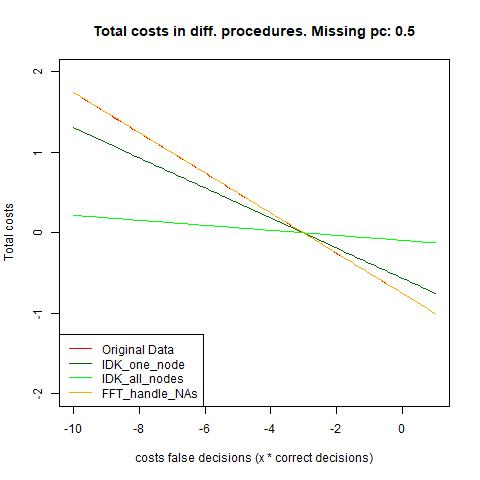
\includegraphics{graphs/diff_procedures_compare.jpg}
\caption{Graph 1: Example for 50\% missings in titanic data. Total costs
for different procedures depended on the relationship of costs of
correct to false decisions (false = -x * correct decision).}
\end{figure}

We optimized for accuracy.

\hypertarget{results}{%
\subsection{Results:}\label{results}}

\begin{enumerate}
\def\labelenumi{\arabic{enumi}.}
\tightlist
\item
  Comparing ``one\_IDK'' performance with the performance of the FFT
  algorithm. The x-axis shows the percentage of missing data in each
  data set, the y-axis displays the costs of wrong decisions (x * -1,
  meaning: the costs of false decisions have to be x times as bad as
  correct decisions for the performance to be better/worse than not
  deciding). Distinct colours represent different data sets.
\end{enumerate}

\begin{figure}
\centering
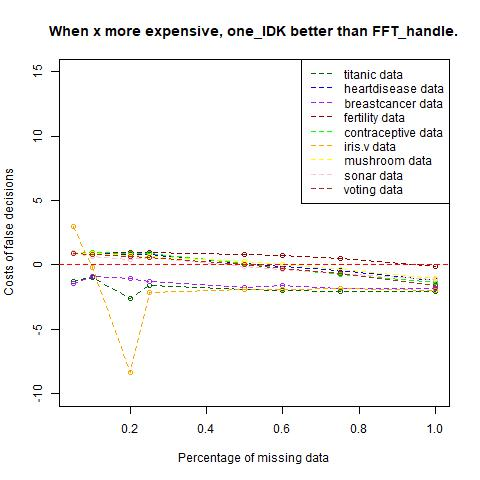
\includegraphics{graphs/acc_one_IDK_overview.jpg}
\caption{Graph 2: Overview. one IDK.}
\end{figure}

\begin{figure}
\centering
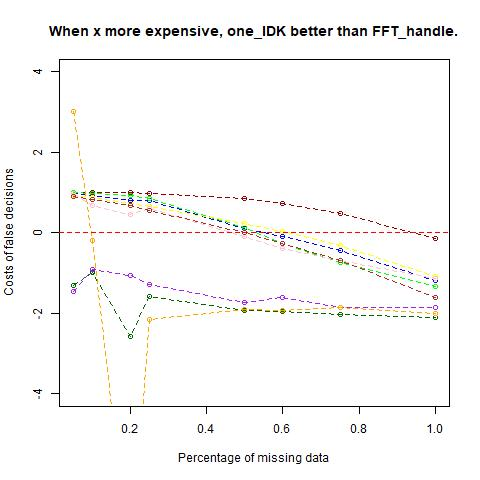
\includegraphics{graphs/acc_one_IDK_see_better.jpg}
\caption{Graph 3: Details. one IDK.}
\end{figure}

\hypertarget{interpretation}{%
\paragraph{Interpretation:}\label{interpretation}}

We have not yet figured out why the performance curve seems to behave
quite similar between some, and really different in between other data
sets. Maybe we can investigate that with correlative calculations
between approximated curves of data set performances and multiple
variables that could theoretically predict the shape of the performance
curve.

\begin{enumerate}
\def\labelenumi{\arabic{enumi}.}
\setcounter{enumi}{1}
\tightlist
\item
  Comparing ``all\_IDK'' performance with the performance of the FFT
  algorithm. The same explanation holds for this graph.
\end{enumerate}

\begin{figure}
\centering
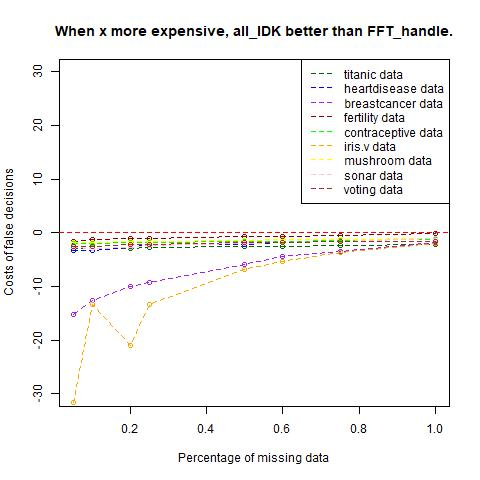
\includegraphics{graphs/acc_all_IDK_overview.jpg}
\caption{Graph 4: Overview. all IDK.}
\end{figure}

\begin{figure}
\centering
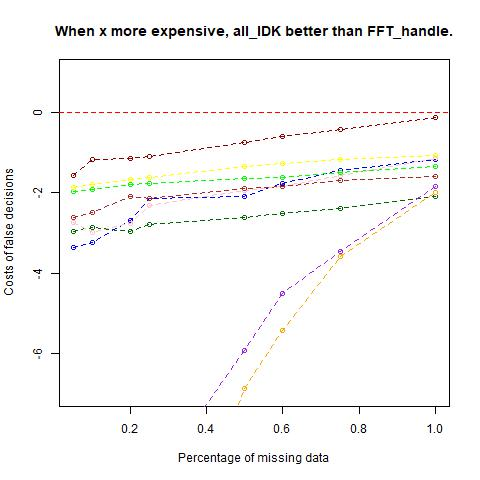
\includegraphics{graphs/acc_all_IDK_better_see.jpg}
\caption{Graph 5: Details. all IDK.}
\end{figure}

\hypertarget{interpretation-1}{%
\paragraph{Interpretation:}\label{interpretation-1}}

Again, we see a similar pattern. In general, most data sets perform
similarly while a few show wildly different patterns. Explanations will
hopefully follow.

Interpreting the results, it seems that the all\_IDK performs worse than
the FFT algorithm in all common sense cases. (With common sense, we mean
the relationship of costs). In contrast, not deciding when all
predictive variables are missing for a case seems to produce better
performances on average for common sense cases. Interestingly, the
trends of how a bigger percentage of NAs in the data sets influences the
performance comparison is antidromic in both cases: The one\_IDK case,
performs much better than FFT if there is a small percentage of NAs and
its comparative advantage shrinks with bigger amounts of NAs, whereas
the all\_IDK option performance comparatively poorly for small
percentages of NAs and improves comparatively with bigger percentages of
NAs. It does however never outperform the other options (in common sense
scenarios). Still, keep in mind that these observations vary greatly in
between data sets due to not yet known factors.

\hypertarget{discussion}{%
\subsection{Discussion:}\label{discussion}}

To further deploy FFTrees algorithms in dichotomous decisions, it should
be considered whether a possibility to not decide when all data is
missing in the decisive variables should be added. In some cases the
data hints that this could yield cheaper total decision costs on average
for some data sets.

\hypertarget{future-research}{%
\subsection{Future research:}\label{future-research}}

Topic one:

\begin{itemize}
\item
  We will attempt to comprehend the patterns governing the varying
  efficacy of different decision rules, whether involving deciding or
  not deciding, across diverse data sets with distinct characteristics.
\item
  We could compare performances when optimizing for bacc.
\end{itemize}

Topic two:

\begin{itemize}
\item
  We will investigate how alternative decision algorithms handle missing
  data.
\item
  Next, we will compare the performance of different algorithms when
  calibrated on complete data sets and subsequently tested with varying
  percentages of missing data.
\item
  We hypothesize that FFTrees exhibit greater robustness in performance
  compared to other algorithms.
\end{itemize}

\hypertarget{further-explorations-which-we-did-but-which-were-not-included-in-this-summary}{%
\subsubsection{Further explorations which we did, but which were not
included in this
summary:}\label{further-explorations-which-we-did-but-which-were-not-included-in-this-summary}}

\begin{itemize}
\item
  Examining performance when permitting compensation---allowing FFTrees
  to construct a more suitable tree in the presence of missing data.
  This consistently showed a better performance but was not further
  investigated since it likely cannot be used in real life easily (when
  data is missing, criterion for good fitting might not be known).
\item
  Exploring the performance loss with increasing percentages of
  missings.
\end{itemize}

Here, we depict the mean results from all utilized data sets:

Example which shows the normalized results of three data sets
(heartdisease, titanic, breastcancer).

\begin{figure}
\centering
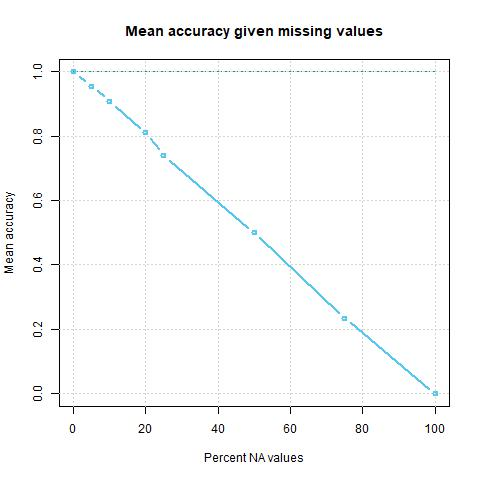
\includegraphics{graphs/meanacc.jpg}
\caption{Graph 6: Normalized mean accuracy, dependent on pc NA in the
data sets.}
\end{figure}

\begin{figure}
\centering
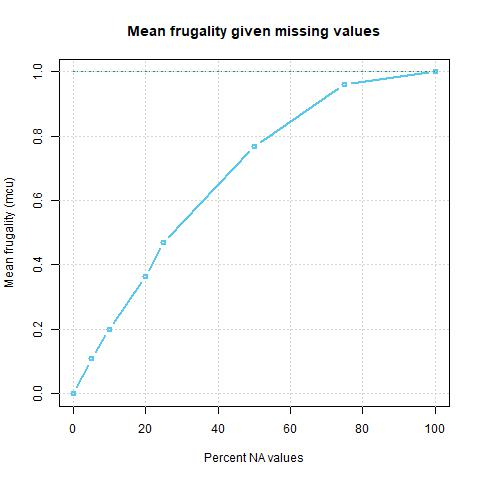
\includegraphics{graphs/meanfrugality.jpg}
\caption{Graph 7: Normalized mean frugality, dependent on pc NA in the
data sets.}
\end{figure}

\end{document}
